\newpage
\section{Are You Getting Stairs?} 
                                  

Most building codes have very specific restrictions on how a staircase
can be designed. Here are typical restrictions:
\begin{enumerate}
\item The stair-step height can be at most $7\frac{3}{4}''$. 
\item The stair-step depth must be at least $10''$.
\item From step-to-step, these dimensions cannot change (in real-life there is a minimum allowed variance for these dimensions). 
\end{enumerate}

\begin{prob} 
If you wish to build a staircase that is $15'$ wide, how tall can it
be?
\end{prob}

\begin{prob} 
If you wish to build a staircase that is $12'$ tall, what is the minimum width that can it
be?
\end{prob}

Allow me to suggest using the following friendly matrix for the
remainder of the problems:
\[
\mat{D}_{s,t}= 
\begin{bmatrix}
s & 0 & 0 \\
0 & t & 0 \\
0 & 0 & 1
\end{bmatrix}
\]
This is a geometric transformation that will dilate a picture by a
scale factor of $s$ in the horizontal direction and a scale factor of
$t$ in the vertical direction. We'll use this to transform a
``generic'' staircase of $n$ stairs to fit our needs:
\[
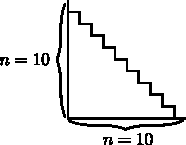
\includegraphics{../graphics/staircase.pdf} 
\]
The upshot is that in essence, to lay a staircase of $n$ stairs that
is up to code in a space that is $w$ feet wide and $h$ feet tall, you
must solve the following equation:
\[
\mat{D}_{s,t}
\begin{bmatrix}
n \\
n \\
1
\end{bmatrix}
= 
\begin{bmatrix}
w \\
h \\
1
\end{bmatrix}
\]
where 
$t\le \frac{31}{48}$ and $s\ge \frac{5}{6}$.

\begin{prob}
Where do the numbers 
\[
\frac{31}{48}\qquad\text{and}\qquad \frac{5}{6}
\]
come from?
\end{prob}


\begin{prob}
Carefully draw an $(s,t)$-plane, with $s$ on the horizontal axis and $t$ on the vertical axis. 
\begin{enumerate}
\item Shade in the region  $t\le \frac{31}{48}$ and $s\ge \frac{5}{6}$.
\item Expand the left-hand side of the following equation: 
\[
\mat{D}_{s,t}
\begin{bmatrix}
n \\ n \\ 1
\end{bmatrix}
= 
\begin{bmatrix}
w \\
h \\
1
\end{bmatrix}
\]
\item Now you should be able to write two equations. In each case, solve for $n$ and set these two equations equal to each other. 
\item Solve for $t$. Now you should have a single equation $t= \dots$.
\item Now you can set values for $w$ and $h$. Set $w = 15$ and $h=11$. Plot your equation on the $(s,t)$-plane---what does this mean?
\end{enumerate}
\end{prob}


\begin{prob}\label{P:Stair}
Suppose you wish to build a staircase that is $15'$ wide and $11'$
tall. What should be the dimensions of each step? How many different
solutions can you find?
\end{prob}

\begin{prob}
Suppose you wish to build a staircase that is $15'$ wide and $10'$
tall. What should be the dimensions of each step? How many different
solutions can you find?
\end{prob}

\begin{prob}
Suppose you wish to build a staircase that is $16'$ wide and $10'$
tall. What should be the dimensions of each step? How many different
solutions can you find?
\end{prob}


\begin{prob}
Smart Sam says he doesn't need matrices to solve
Problem \ref{P:Stair}. Instead, he says:
\begin{quote}
First you take the height of the staircase, $11'$ and divide it by
$31/48'$ to get $18$. Now take $15'$ and divide by $18$ to get
$5/6'$. So you have $18$ steps that are $5/6'$ deep and $31/48'$ tall.
\end{quote}
His arithmetic seems a bit strange to me, what is he doing?  Is his
solution different from what we did above? Hint: There are at least
two errors in his solution, one that is minor and another that is
major.
\end{prob}
